%!TEX root = ComputerScienceOne.tex

%Loops - exercises

\section{Exercises}

\begin{exer}
Write a for-loop and a while-loop that accomplishes each of the following.
\begin{enumerate}
  \item[(a)] Prints all integers 1 thru 100 on the same line delimited by a single space
  \item[(b)] Prints all even integers 0 up to $n$ in reverse order
  \item[(c)] A list of integers divisible by 3 between $a$ and $b$ where $a, b$ are parameters or inputs
  \item[(d)] Prints all positive powers of two up to $2^{30}$ : $1, 2, 4, \ldots, 1073741824$ one value per line (try computing up to $2^{31}$ and $2^{32}$ and discern reasons for why it may fail)
  \item[(e)] Prints all even integers 2 thru 200 on 10 different lines (10 numbers on each line) \emph{in reverse order}
  \item[(f)] Prints the following pattern of numbers (hint: use two nested loops; the result can be computed using some value of $i + 10j$)
\end{enumerate}

\begin{minted}{text}
 11  21  31  41  51  61  71  81  91 101
 12  22  32  42  52  62  72  82  92 102
 13  23  33  43  53  63  73  83  93 103
 14  24  34  44  54  64  74  84  94 104
 15  25  35  45  55  65  75  85  95 105
 16  26  36  46  56  66  76  86  96 106
 17  27  37  47  57  67  77  87  97 107
 18  28  38  48  58  68  78  88  98 108
 19  29  39  49  59  69  79  89  99 109
 20  30  40  50  60  70  80  90 100 110
   \end{minted}
\end{exer}

\begin{exer}
Civil engineers have come up with two different models on how a city's 
population will grow over the next several years.  The first projection assumes
a 10\% annual growth rate while the second projection assumes a linear growth
rate of 50,000 additional citizens per year.  Write a program to project the
population growth under both models.  Take, as input, the initial population of
the city along with a number of years to project the population.

In addition, compute how many years it would take to \emph{double} the population
under each model.
\end{exer}

\begin{exer}
Write a loan program similar to the amortization schedule program we developed in 
Section \ref{subsection:loanAmortization}.  However, give the user an option to 
specify an \emph{extra} monthly payment amount in order to pay off the loan
early.  Calculate how much quicker the loan gets paid off and how much they
save in interest.  
\end{exer}

%\begin{exer}
%Write a Program to create a table containing a customized loan amortization table. Your program will
%prompt the user to enter the amount borrowed (the $\emph{principal}$), the annual interest rate(format: $\texttt{5.05}$ is
%5.5$\%$), and the number of monthly payments ($\emph{n}$). To calculate the monthly payment, use the following formula:
%$$ {payment} = \frac{iP}{1 - (1 + i)^{-n}} $$
%where
%\begin{itemize}
%  \item \emph{P} is the initial principal amount
%  \item \emph{i} is the monthly interest rate ($\frac{1}{12}$ of the APR)
%  \item \emph{n} is the total number of payments (payment periods)
%\end{itemize}
%Note that this payment must be rounded to the nearest cent. After the payment has been rounded to the nearest cent,
%the program will create a table that looks like the following.
%\begin{minted}{text}
%Principal: $1000.00
%Annual Interest Rate: 9.00 %
%Term: 6 months
%Monthly Payment: $171.07
%Payment     Interest       Principal        Balance
%1           $   7.50        $ 163.57       $ 836.43
%2           $   6.27        $ 164.80       $ 671.63
%3           $   5.04        $ 166.03       $ 505.60
%4           $   3.79        $ 167.28       $ 338.32
%5           $   2.54        $ 168.53       $ 169.79
%6           $   1.27        $ 169.79       $   0.00
%Final Payment: $171.06
%\end{minted}
%
%Each month, part of the payment is applied to the interest and the rest is applied to the principal
%Because the payment and each month's interest rate are rounded, the final payment will be a bit different
%and must be calculated as the sum of the final interest payment and the final principal balance.
%\end{exer}

\begin{exer}
The rate of decay of a radioactive
isotope is given in terms of its half-life $H$, the time lapse required
for the isotope to decay to one-half of its original mass. For example,
the isotope Strontium-90 ($^{90}Sr$) has a half-life of 28.9 years.  If
we start with 10kg of Strontium-90 then 28.9 years later you 
would expect to have only 5kg of Strontium-90 (and 5kg
of Yttrium-90 and Zirconium-90, isotopes which Strontium-90 decays
into).

Write a program that takes the following input:
\begin{itemize}
  \item Atomic Number (integer)
  \item Element Name
  \item Element Symbol
  \item $H$ (half-life of the element)
  \item $m$, an initial mass in grams
\end{itemize}

Your program will then produce a table detailing the amount of the element
that remains after each year until less than 50\% of the original amount remains.
This amount can be computed using the following formula:
  $$r = m \times \left(\frac{1}{2}\right)^{(y/H)}$$
$y$ is the number of years
elapsed, and $H$ is the half-life of the isotope in years.

For example, using your program on Strontium-90 (symbol: Sr, atomic number: 38)
with a half-life of 28.9 years and an initial amount of 10 grams would produce a table something like:
\begin{minted}{text}
 Strontium-90 (38-Sr)
Elapsed Years    Amount
-------------------------
-                10g
1                9.76g
2                9.53g
3                9.30g
...
28               5.11g
29               4.99g
\end{minted}
\end{exer}

\begin{exer}
In this exercise, you will develop a program that assists people in saving for a retirement
using a tax-deferred 401k program.  

Your application will allow a user to enter the following inputs:
\begin{itemize}
  \item An initial starting balance
  \item A monthly contribution amount (we'll assume its the same over the life of the savings plan)
  \item An (average) annual rate of return
  \item An (average) annual rate of inflation
\end{itemize}

In addition, your program will allow a user to choose between two different scenarios:
\begin{itemize}
  \item The first will allow the user to input a number of \emph{years} left until retirement.  
  	It will then compute a monthly savings table which will be a projection out to that many years.
  \item The second will take a \emph{target} dollar amount and compute a monthly savings
  	table until the account balance has reached this target dollar amount.
\end{itemize}

The monthly interest rate should be inflation-adjusted.  The inflation-adjusted 
rate of return can be computed with the following formula.
  $$\frac{1 + \textrm{rate of return}}{1+\textrm{inflation rate}} - 1$$
To get the monthly rate, simply divide by 12.  Each month, interest is applied to the balance at this 
rate along with the monthly contribution amount.

An example: if we start with \$10,000 and contribute \$500 monthly with a return rate of 9\% and
an inflation rate of 1.2\%, the first few lines of our table would something like the following.

\begin{minted}{text}
Payment     Interest Earned  Contribution   Balance
1           $   64.23        $ 500.00       $ 10564.23
2           $   67.85        $ 500.00       $ 11132.08
3           $   71.50        $ 500.00       $ 11703.58
4           $   75.17        $ 500.00       $ 12278.75
...
\end{minted}

\end{exer}

%applied math type problems

\begin{exer}
Write a program that computes various statistics on a collection of numbers that can
be read in from the command line, as command line arguments, or via other means.
In particular, given $n$ numbers, 
  $$x_1, x_2, \ldots, x_n$$
your program should compute the following statistics:
\begin{itemize}
  \item The minimum number
  \item The maximum number
  \item The mean,
   $$\mu = \frac{1}{n} \sum_{i=1}^n x_i$$
  \item The variance,
   $$\sigma^2 = \frac{1}{n} \sum_{i=1}^n (x_i - \mu)^2$$
  \item And the standard deviation,
   $$\sigma = \sqrt{\frac{1}{n} \sum_{i=1}^n (x_i - \mu)^2}$$
\end{itemize}
where $n$ is the number of numbers that was provided.  For example, with the numbers, 
  $$3.14, 2.71, 42, 3, 13$$
your output should look something like:

\begin{minted}{text}
Minimum:      2.71
Maximum:     42.00
Mean:        12.77
Variance:   228.77
Standard
Deviation:   15.13
\end{minted}
\end{exer}

\begin{exer}
\label{exercise:loops:gcd}
The ancient Greek mathematician Euclid developed a method for finding
the greatest common divisor of two positive integers, $a$ and $b$. His method is
as follows:
\begin{enumerate}
  \item If the remainder of $a/b$ is 0 then $b$ is the greatest
      common divisor.
  \item If it is not 0, then find the remainder $r$ of $a/b$ and
      assign $b$ to $a$ and the remainder $r$ to $b$.
  \item Return to step (1) and repeat the process.
\end{enumerate}
Write a program that uses a function to perform this procedure. Display
the two integers and the greatest common divisor.
\end{exer}

%numerical analysis type math

\begin{exer}
Write a program to estimate the value of $e \approx 2.718281\ldots$ using the series: 
  $$e = \sum_{k=0}^{\infty} \frac{1}{k!}$$
Obviously, you will need to restrict the summation to a finite number of $n$ terms.
\end{exer}

\begin{exer}
The value of ${\pi}$ can be expressed by the following infinite series:
 $$ {\pi} = 4  \cdot \left( 1 - \frac{1}{3} + \frac{1}{5} - \frac{1}{7} + \frac{1}{9} - \frac{1}{11} + \frac{1}{13} - \cdots \right)$$
An approximation can be made by taking the first $n$ terms of the series.  For $n = 4$, the approximation is
 $$\pi \approx 4 \cdot \left( 1 - \frac{1}{3} + \frac{1}{5} - \frac{1}{7} \right) = 2.8952$$
Write a program that takes $n$ as input and outputs an approximation of $\pi$ according to the
series above.
\end{exer}

\begin{exer}
The sine function can be approximated using the following Taylor series.
  $$\sin{(x)} = \sum_{i=0}^{\infty} \frac{(-1)^i}{(2i+1)!} x^{2i+1} = x - \frac{x^3}{3!} + \frac{x^5}{5!} - \cdots$$
Write a function that takes $x$ and $n$ as inputs and approximates $\sin{x}$ by computing the first $n$
terms in the series above.
\end{exer}

\begin{exer}
One way to compute $\pi$ is to use Machin's formula:
  $$\frac{\pi}{4} = 4 \arctan{\frac{1}{5}} - \arctan{\frac{1}{239}}$$
To compute the $\arctan$ function, you could use the following series:
  $$\arctan{x} = \frac{x}{1} - \frac{x^3}{3} + \frac{x^5}{5} - \frac{x^7}{7} + \cdots = \sum_{i=0}^{\infty} \frac{(-1)^i}{2k+1} x^{2i + 1}$$
Write a program to estimate $\pi$ using these formulas but allowing
the user to specify how many terms to use in the series to compute it.
Compare the estimate with the built-in definition of $\pi$ in your language.  
\end{exer}

\begin{exer}
The \emph{arithmetic-geometric} mean of two numbers $x, y$, denoted $M(x, y)$ 
(or $\mathrm{agm}(x, y)$) can be computed iteratively as follows.  Initially, 
$a_1 = \frac{1}{2}(x + y)$ and $g_1 = \sqrt{xy}$ (i.e. the normal arithmetic and 
geometric means).  Then, compute
  $$\begin{array}{rcl}
    a_{n+1} & = & \frac{1}{2}(a_n+g_n) \\
    g_{n+1} & = & \sqrt{a_n g_n}
    \end{array}$$
The two sequences will converge to the same number which is the arithmetic-geometric 
mean of $x, y$.  Obviously we cannot compute an infinite sequence, so we compute until
$|a_n - g_n| < \epsilon$ for some small number $\epsilon$.
\end{exer}

\begin{exer}
The integral of a function is a measure of the area under its curve.  One numerical method for 
computing the integral of a function $f(x)$ on an interval $[a, b]$ is the \emph{rectangle} rule.
Specifically, an interval $[a, b]$ is split up into $n$ equal subintervals of size
$h = \frac{b-a}{n}$.  Then the integral is approximated by computing:
  $$\int_{a}^{b} f(x) dx \approx \sum_{i=0}^{n-1} f(a + ih) \cdot h$$
Write a program to approximate an integral using the rectangle method.  For this particular exercise you 
will integrate the function
  $$f(x) = \frac{\sin{x}}{x}$$
For reference, the function is depicted in Figure \ref{fig:sinxx}.  Write a program that will
read the end points $a, b$ and the number of subintervals $n$ and computes the integral 
of $f$ using the rectangle method.  It should then output the approximation.

\begin{figure}[h]
\centering
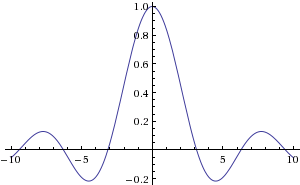
\includegraphics[scale=0.65]{images/sinxx}
\caption{Plot of $f(x) = \frac{\sin{x}}{x}$}
\label{fig:sinxx}
\end{figure}
\end{exer}

\begin{exer}
Another way to compute an integral is to a technique called \emph{Monte Carlo Integration}, 
a randomized numerical integration method.

Given the interval $[a, b]$, we enclose the function in a region of interest with a rectangle of a known
area $A_r$.  We then randomly select $n$ points within the rectangle and count the number of random
points that are within the function's curve.  If $m$ of the $n$ points are within the curve, we can estimate
the integral to be
 $$\int_a^b \! f(x) \, \mathrm{d} x \approx \frac{m}{n}A_r$$

Consider again the function $f(x) = \frac{\sin(x)}{x}$.  Note that the global maximum and 
minimum of this function are 1 and $\approx -0.2172$ respectively.
Therefore, we can also restrict the rectangle along the $y$-axis from $-.25$ to $1$.  That is, the lower
left of the rectangle will be $(a, -.25)$ and the upper right will be $(b, 1)$ for a known area of
 $$A_r = |a - b| \times 1.25$$
Figure \ref{fig:sinxxRect} illustrates the rectangle for the interval $[-5, 5]$.

\begin{figure}[h]
\centering
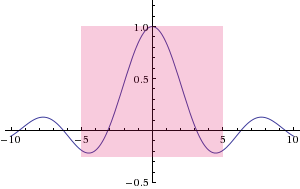
\includegraphics[scale=.75]{images/sinxxRect.png}
\caption{A rectangle for the interval $[-5, 5]$.}
\label{fig:sinxxRect}
\end{figure}

Write a program that will takes as input interval values $a, b$, and an integer $n$ and 
perform a Monte Carlo estimate of the integral of the function above.  Realize that this 
is just an approximation and it is randomized so your answers may not match exactly
and may be different on various executions of your program.  Take care that you handle 
points within the curve but under the $x$-axis correctly.
\end{exer}


\begin{exer}
Consider a ball trapped in a 2-D box.  Suppose that it has an initial position $(x, y)$ within the box
(the box's dimensions are specified by its lower left $(x_\ell, y_\ell)$ and an upper right $(x_r, y_r)$ points)
along with an initial angle of travel $\theta$ in the range $[0, 2\pi)$.  As the ball travels in this direction it
will eventually collide with one of the sides of the box and bounce off.  For this model, we will assume no loss of velocity
(it keeps going) and its angle of reflection is perfect.  

Write a program that takes as input, $x, y, \theta, x_\ell, y_\ell, x_r, y_r$, and an integer $n$
and computes the first $n-1$ Euclidean points on the box's perimeter that the ball bounces off of in its
travel (include the initial point in your printout for a total of $n$ points).  You may assume that the input will always be ``good'' (the ball will always begin somewhere inside the box
and the lower left and upper right points will not be reversed).

As an example, consider the inputs: 
$$x = 1, y=1, \theta = .392699, x_\ell = 0, y_\ell = 0, x_r = 4, y_r = 3,  n = 20$$
Starting at $(1, 1)$, the ball travels up and to the right bouncing off the right wall.  Figure 
\ref{fig:bouncyBall} illustrates this and the subsequent bounces back and forth.

\begin{figure}[h]
\centering
%\documentclass{article}
%\usepackage{tikz}
%\usetikzlibrary{arrows.meta}
%\begin{document}

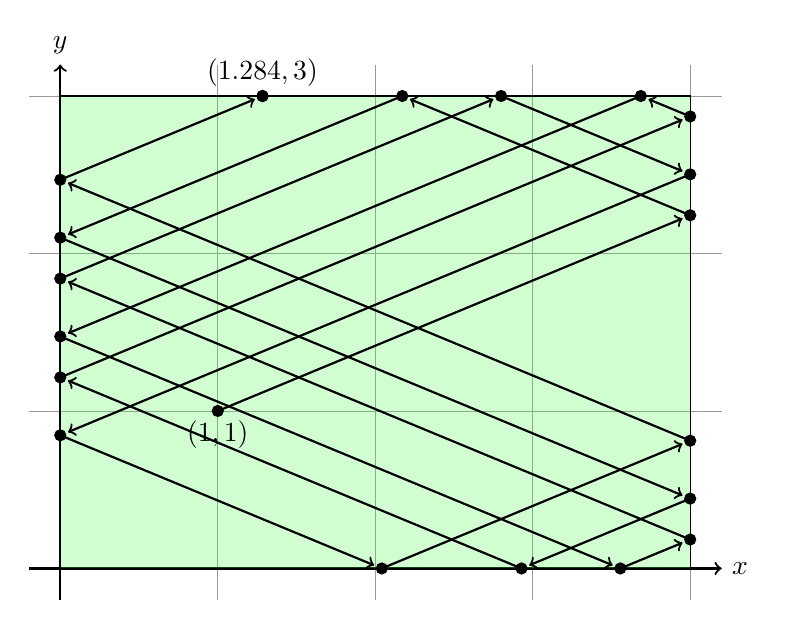
\begin{tikzpicture}[scale=2.0]
  \draw[step=1.0cm,black!40!white,very thin] (-0.2,-0.2) grid (4.2,3.2); %
  \draw[thick,->] (0, -0.2) -- (0, 3.2) node[above] {$y$};%
  \draw[thick,->] (-0.2, 0) -- (4.2, 0) node[right] {$x$};%

  \filldraw[fill=green!70!white,fill opacity=.25] (0, 0) rectangle (4,3);

  \draw[fill] (1, 1) circle (1pt) node[below] {$(1, 1)$};
  \draw[fill] (4.000000, 2.242641) circle (1pt);
  \draw[->,shorten >=3pt,thick] (1.000000,1.000000) -- (4.000000,2.242641);
  \draw[fill] (2.171573, 3.000000) circle (1pt);
  \draw[->,shorten >=3pt,thick] (4.000000,2.242641) -- (2.171573,3.000000);
  \draw[fill] (0.000000, 2.100505) circle (1pt);
  \draw[->,shorten >=3pt,thick] (2.171573,3.000000) -- (0.000000,2.100505);
  \draw[fill] (4.000000, 0.443651) circle (1pt);
  \draw[->,shorten >=3pt,thick] (0.000000,2.100505) -- (4.000000,0.443651);
  \draw[fill] (2.928932, 0.000000) circle (1pt);
  \draw[->,shorten >=3pt,thick] (4.000000,0.443651) -- (2.928932,0.000000);
  \draw[fill] (0.000000, 1.213203) circle (1pt);
  \draw[->,shorten >=3pt,thick] (2.928932,0.000000) -- (0.000000,1.213203);
  \draw[fill] (4.000000, 2.870058) circle (1pt);
  \draw[->,shorten >=3pt,thick] (0.000000,1.213203) -- (4.000000,2.870058);
  \draw[fill] (3.686291, 3.000000) circle (1pt);
  \draw[->,shorten >=3pt,thick] (4.000000,2.870058) -- (3.686291,3.000000);
  \draw[fill] (0.000000, 1.473088) circle (1pt);
  \draw[->,shorten >=3pt,thick] (3.686291,3.000000) -- (0.000000,1.473088);
  \draw[fill] (3.556349, 0.000000) circle (1pt);
  \draw[->,shorten >=3pt,thick] (0.000000,1.473088) -- (3.556349,0.000000);
  \draw[fill] (4.000000, 0.183766) circle (1pt);
  \draw[->,shorten >=3pt,thick] (3.556349,0.000000) -- (4.000000,0.183766);
  \draw[fill] (0.000000, 1.840620) circle (1pt);
  \draw[->,shorten >=3pt,thick] (4.000000,0.183766) -- (0.000000,1.840620);
  \draw[fill] (2.798990, 3.000000) circle (1pt);
  \draw[->,shorten >=3pt,thick] (0.000000,1.840620) -- (2.798990,3.000000);
  \draw[fill] (4.000000, 2.502525) circle (1pt);
  \draw[->,shorten >=3pt,thick] (2.798990,3.000000) -- (4.000000,2.502525);
  \draw[fill] (0.000000, 0.845671) circle (1pt);
  \draw[->,shorten >=3pt,thick] (4.000000,2.502525) -- (0.000000,0.845671);
  \draw[fill] (2.041631, 0.000000) circle (1pt);
  \draw[->,shorten >=3pt,thick] (0.000000,0.845671) -- (2.041631,0.000000);
  \draw[fill] (4.000000, 0.811183) circle (1pt);
  \draw[->,shorten >=3pt,thick] (2.041631,0.000000) -- (4.000000,0.811183);
  \draw[fill] (0.000000, 2.468037) circle (1pt);
  \draw[->,shorten >=3pt,thick] (4.000000,0.811183) -- (0.000000,2.468037);
  \draw[fill] (1.284271, 3.000000) circle (1pt);
  \draw[->,shorten >=3pt,thick] (0.000000,2.468037) -- (1.284271,3.000000);

  \draw[fill] (1.284, 3) circle (1pt) node[above] {$(1.284, 3)$};  

\end{tikzpicture}

%\end{document}


\caption{Follow the bouncing ball}
\label{fig:bouncyBall}
\end{figure}

Your output should simply be the points and should look something like the following.

\begin{minted}{text}
(1.000000, 1.000000)
(4.000000, 2.242640)
(2.171572, 3.000000)
(0.000000, 2.100506)
(4.000000, 0.443652)
(2.928929, 0.000000)
(0.000000, 1.213202)
(4.000000, 2.870056)
(3.686287, 3.000000)
(0.000000, 1.473090)
(3.556355, 0.000000)
(4.000000, 0.183764)
(0.000000, 1.840617)
(2.798998, 3.000000)
(4.000000, 2.502529)
(0.000000, 0.845675)
(2.041640, 0.000000)
(4.000000, 0.811179)
(0.000000, 2.468033)
(1.284282, 3.000000)
\end{minted}

\end{exer}

\begin{exer}
An integer $n \geq 2$ is \emph{prime} if its only divisors are $1$ and itself, $n$.  For example, $2, 3, 5, 7, 11, \ldots$
are primes.  Write a program that outputs all prime numbers $2$ up to $m$ where $m$ is read as input.
\end{exer}

\begin{exer}
An integer $n \geq 2$ is \emph{prime} if the only integers that evenly divide it are $1$ and $n$ itself, 
otherwise it is \emph{composite}.  The \emph{prime factorization} of an integer is a list of its prime divisors 
along with their multiplicities.  For example, the prime decomposition of $188,760$ is:
  $$188,760 = 2 \cdot 2 \cdot 2 \cdot 3 \cdot 5 \cdot 11 \cdot 11 \cdot 13$$
Write a program that takes an integer $n$ as input and outputs the prime factorization of $n$.
If $n$ is invalid, an appropriate error message should be displayed instead.  Your output should look 
something like the following.
\begin{minted}{text}
1001 = 7 * 11 * 13
\end{minted}
\end{exer}

\begin{exer} 
One way of estimating $\pi$ is to randomly sample points within a $2 \times 2$ square centered
at the origin.  If the distance between the randomly chosen point $(x, y)$ and the origin is less than or
equal to 1, then the point lies inside the unit circle centered at the origin and we count it.  If the 
point lies outside the circle then we can ignore it.  
\begin{figure}[h]
\centering
%\documentclass{article}
%\usepackage{tikz}
%\begin{document}

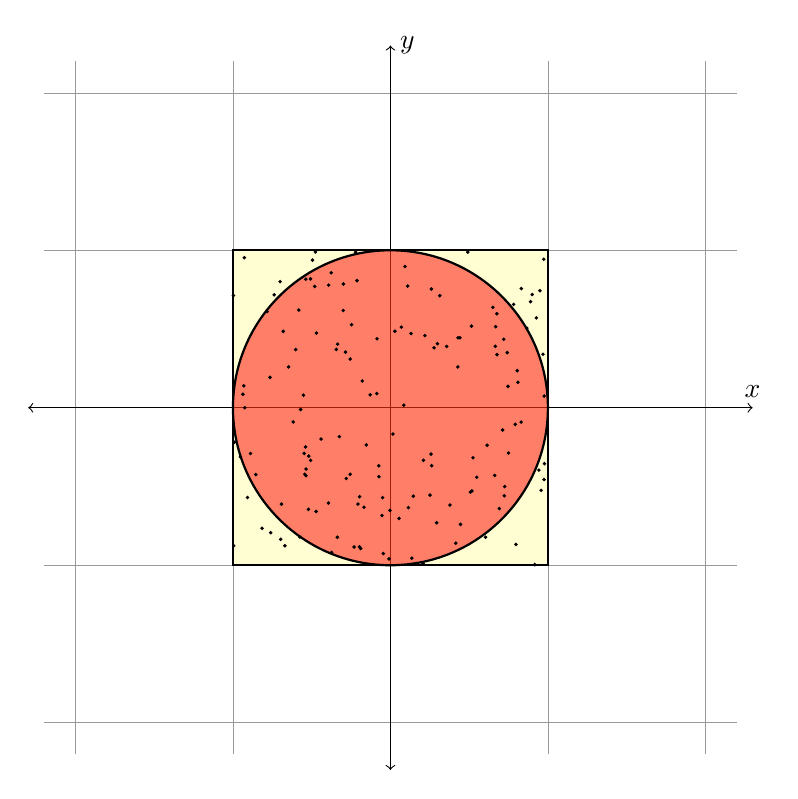
\begin{tikzpicture}[scale=2.0]
  \draw[step=1.0cm,black!40!white,very thin] (-2.2,-2.2) grid (2.2,2.2); %
  \draw[<->] (0, -2.3) -- (0, 2.3) node[right] {$y$};%
  \draw[<->] (-2.3, 0) -- (2.3, 0) node[above] {$x$};%

  \filldraw[fill=yellow!70!white,thick,fill opacity=.25] (-1, -1) rectangle (1,1);
  \filldraw[fill=red,thick,fill opacity=.5] (0, 0) circle (1);

  \fill(-0.179025, 0.170052) circle(.35pt);
  \fill(-0.230483, -0.884416) circle(.35pt);
  \fill(0.440984, 0.444861) circle(.35pt);
  \fill(-0.086282, 0.089922) circle(.35pt);
  \fill(0.749824, -0.287103) circle(.35pt);
  \fill(0.782099, 0.656653) circle(.35pt);
  \fill(0.084703, 0.016307) circle(.35pt);
  \fill(-0.544334, -0.422176) circle(.35pt);
  \fill(-0.575099, -0.820715) circle(.35pt);
  \fill(-0.927591, 0.952768) circle(.35pt);
  \fill(-0.393389, -0.605339) circle(.35pt);
  \fill(-0.581804, 0.620439) circle(.35pt);
  \fill(-0.085225, 0.438428) circle(.35pt);
  \fill(0.676509, 0.337266) circle(.35pt);
  \fill(0.866596, 0.505712) circle(.35pt);
  \fill(-0.952575, -0.312428) circle(.35pt);
  \fill(-0.324235, -0.183058) circle(.35pt);
  \fill(-0.196845, -0.883251) circle(.35pt);
  \fill(-0.738196, 0.716873) circle(.35pt);
  \fill(0.206670, -0.988372) circle(.35pt);
  \fill(-0.570230, -0.011231) circle(.35pt);
  \fill(0.668280, 0.514473) circle(.35pt);
  \fill(-0.994924, -0.876053) circle(.35pt);
  \fill(-0.907703, -0.570023) circle(.35pt);
  \fill(-0.696768, -0.835294) circle(.35pt);
  \fill(-0.617255, -0.090158) circle(.35pt);
  \fill(-0.440633, -0.199060) circle(.35pt);
  \fill(-0.469719, 0.474141) circle(.35pt);
  \fill(-0.760632, -0.793210) circle(.35pt);
  \fill(-0.188592, -0.894036) circle(.35pt);
  \fill(0.712502, -0.141167) circle(.35pt);
  \fill(-0.206464, -0.611733) circle(.35pt);
  \fill(0.675775, 0.596692) circle(.35pt);
  \fill(-0.494985, 0.937579) circle(.35pt);
  \fill(0.313565, 0.711686) circle(.35pt);
  \fill(0.949207, 0.743335) circle(.35pt);
  \fill(-0.299545, 0.617487) circle(.35pt);
  \fill(0.257808, -0.294469) circle(.35pt);
  \fill(0.741434, 0.350105) circle(.35pt);
  \fill(0.135507, -0.955335) circle(.35pt);
  \fill(0.514811, 0.518252) circle(.35pt);
  \fill(-0.045492, -0.925822) circle(.35pt);
  \fill(-0.680808, 0.484789) circle(.35pt);
  \fill(0.548319, -0.441440) circle(.35pt);
  \fill(0.691579, -0.640273) circle(.35pt);
  \fill(-0.335475, 0.404081) circle(.35pt);
  \fill(0.218559, 0.458061) circle(.35pt);
  \fill(0.792347, -0.105666) circle(.35pt);
  \fill(0.054753, -0.702637) circle(.35pt);
  \fill(-0.168087, -0.631682) circle(.35pt);
  \fill(-0.990951, -0.218880) circle(.35pt);
  \fill(-0.888347, -0.290497) circle(.35pt);
  \fill(-0.601393, 0.369461) circle(.35pt);
  \fill(0.415034, -0.859959) circle(.35pt);
  \fill(-0.280434, -0.449458) circle(.35pt);
  \fill(-0.815294, -0.765623) circle(.35pt);
  \fill(-0.931206, 0.139214) circle(.35pt);
  \fill(-0.691446, -0.612014) circle(.35pt);
  \fill(-0.375998, 0.856873) circle(.35pt);
  \fill(-0.053454, -0.684419) circle(.35pt);
  \fill(-0.783400, 0.611071) circle(.35pt);
  \fill(0.719662, 0.435159) circle(.35pt);
  \fill(0.069132, 0.512009) circle(.35pt);
  \fill(-0.670507, -0.876115) circle(.35pt);
  \fill(0.809372, 0.161406) circle(.35pt);
  \fill(-0.507797, 0.818421) circle(.35pt);
  \fill(0.942526, -0.396145) circle(.35pt);
  \fill(-0.472076, -0.658867) circle(.35pt);
  \fill(0.973316, 0.942958) circle(.35pt);
  \fill(-0.518827, -0.307118) circle(.35pt);
  \fill(-0.506500, -0.334121) circle(.35pt);
  \fill(-0.072741, -0.437706) circle(.35pt);
  \fill(0.805093, 0.235813) circle(.35pt);
  \fill(-0.049720, -0.570904) circle(.35pt);
  \fill(0.092686, 0.896826) circle(.35pt);
  \fill(-0.255324, 0.309286) circle(.35pt);
  \fill(0.507897, -0.535662) circle(.35pt);
  \fill(-0.255555, -0.422972) circle(.35pt);
  \fill(0.976347, 0.073938) circle(.35pt);
  \fill(-0.299087, 0.785719) circle(.35pt);
  \fill(-0.764656, 0.193116) circle(.35pt);
  \fill(0.604140, -0.822130) circle(.35pt);
  \fill(0.796971, -0.867936) circle(.35pt);
  \fill(-0.480998, 0.770288) circle(.35pt);
  \fill(-0.924978, 0.000176) circle(.35pt);
  \fill(-0.536830, -0.431478) circle(.35pt);
  \fill(0.666055, 0.390429) circle(.35pt);
  \fill(0.130816, 0.471148) circle(.35pt);
  \fill(-0.373758, -0.918905) circle(.35pt);
  \fill(0.900244, 0.718929) circle(.35pt);
  \fill(0.977921, -0.355080) circle(.35pt);
  \fill(0.028215, 0.485818) circle(.35pt);
  \fill(0.109258, 0.772660) circle(.35pt);
  \fill(-0.937154, 0.085605) circle(.35pt);
  \fill(-0.153402, -0.236241) circle(.35pt);
  \fill(-0.128675, 0.081942) circle(.35pt);
  \fill(0.956875, -0.524535) circle(.35pt);
  \fill(0.259812, 0.753846) circle(.35pt);
  \fill(-0.392472, 0.778814) circle(.35pt);
  \fill(0.524133, -0.317449) circle(.35pt);
  \fill(-0.221010, 0.987303) circle(.35pt);
  \fill(0.251073, -0.554955) circle(.35pt);
  \fill(0.377732, -0.618111) circle(.35pt);
  \fill(0.916193, -0.996025) circle(.35pt);
  \fill(-0.537016, 0.816437) circle(.35pt);
  \fill(0.722903, -0.559095) circle(.35pt);
  \fill(-0.538643, -0.248882) circle(.35pt);
  \fill(0.926722, 0.570615) circle(.35pt);
  \fill(-0.476222, 0.989568) circle(.35pt);
  \fill(-0.343779, 0.370376) circle(.35pt);
  \fill(-0.246672, 0.527545) circle(.35pt);
  \fill(-0.547683, -0.289798) circle(.35pt);
  \fill(-0.996990, 0.712129) circle(.35pt);
  \fill(-0.535952, -0.389462) circle(.35pt);
  \fill(0.490943, 0.988182) circle(.35pt);
  \fill(0.293089, -0.730067) circle(.35pt);
  \fill(0.975485, -0.455838) circle(.35pt);
  \fill(-0.285022, 0.353217) circle(.35pt);
  \fill(-0.073950, -0.368829) circle(.35pt);
  \fill(0.357192, 0.389034) circle(.35pt);
  \fill(-0.552392, 0.080095) circle(.35pt);
  \fill(0.829939, -0.091035) circle(.35pt);
  \fill(0.831214, 0.756661) circle(.35pt);
  \fill(-0.520420, -0.645008) circle(.35pt);
  \fill(0.746230, 0.135801) circle(.35pt);
  \fill(0.725367, -0.500443) circle(.35pt);
  \fill(-0.336654, -0.822315) circle(.35pt);
  \fill(0.209760, -0.333644) circle(.35pt);
  \fill(0.889814, 0.673808) circle(.35pt);
  \fill(0.276895, 0.380757) circle(.35pt);
  \fill(0.661990, -0.430016) circle(.35pt);
  \fill(0.650690, 0.637475) circle(.35pt);
  \fill(0.114146, -0.634332) circle(.35pt);
  \fill(-0.009308, -0.959804) circle(.35pt);
  \fill(-0.003161, -0.652116) circle(.35pt);
  \fill(0.429230, 0.444447) circle(.35pt);
  \fill(0.427980, 0.259169) circle(.35pt);
  \fill(-0.646589, 0.259193) circle(.35pt);
  \fill(0.015831, -0.167009) circle(.35pt);
  \fill(0.614185, -0.237939) circle(.35pt);
  \fill(0.968792, 0.339552) circle(.35pt);
  \fill(0.261618, -0.367862) circle(.35pt);
  \fill(0.517237, -0.528622) circle(.35pt);
  \fill(0.298494, 0.407051) circle(.35pt);
  \fill(-0.854814, -0.424611) circle(.35pt);
  \fill(-0.212193, 0.807176) circle(.35pt);
  \fill(0.145373, -0.561503) circle(.35pt);
  \fill(0.444651, -0.740482) circle(.35pt);
  \fill(-0.195835, -0.564656) circle(.35pt);
  \fill(-0.700286, 0.801004) circle(.35pt);



\end{tikzpicture}

%\end{document}


\caption{Sampling points in a circle}
\label{fig:circleSample}
\end{figure}
If we sample $n$ points and $m$ of them lie within the circle, then $\pi$ can be estimated as
 $$\pi \approx \frac{4m}{n}$$
Given a point $(x, y)$, its distance from the origin is simply
  $$\sqrt{x^2 + y^2}$$
This idea is illustrated in Figure \ref{fig:circleSample}.  Example code is given to randomly generate 
numbers within a bound.  Write a program that takes an integer $n$ as input and 
randomly samples $n$ points within the $2 \times 2$ square and outputs an approximation of $\pi$.

Of course, you'll need a way to generate random numbers within the range $[-1, 1]$.  Since you are
using some randomization, the result is just an \emph{approximation} and may not match exactly or
even be the same between two different runs of your program.
\end{exer}

\begin{exer}
A regular polygon is a polygon that is equiangular.  That is, it has $n$ sides and $n$ points whose angle from the
center are all equal in measure.  Examples for $n = 3$ through $n = 8$ can be found in Figure \ref{fig:regularPolygons}.

\begin{figure}[h]
\centering
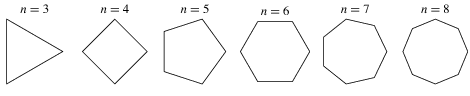
\includegraphics[scale=0.60]{images/regularPolygons}
%\input{regularPolygons}
\caption{Regular polygons}
\label{fig:regularPolygons}
\end{figure}

Write a program that takes $n$ and a radius $r$ as inputs and computes the points
of a regular $n$-sided polygon centered at the origin $(0,0)$.  Each point should be distance $r$
from the origin and the first point should lie on the positive $x$-axis.  Each subsequent point should be
at an angle $\theta$ equal to $\frac{2\pi}{n}$ from the previous point.  Recall that given the
polar coordinates $\theta, r$ we can convert to cartesian coordinates $(x, y)$ using the following.
$$\begin{array}{rcl}
 x & = & r \cdot \cos{\theta} \\
 y & = & r \cdot \sin{\theta}
\end{array}$$
Your program should be robust enough to check for invalid inputs.  If invalid, an error message should
be printed and the program should exit.

For example, running your program with $n = 5, r = 6$ should produce the points of a 
pentagon with ``radius'' $6$.  The output should look something like:

\begin{minted}{text}
Regular 5-sided polygon with radius 6.0:
(6.0000, 0.0000)
(1.8541, 5.7063)
(-4.8541, 3.5267)
(-4.8541, -3.5267)
(1.8541, -5.7063)
\end{minted}

\end{exer}

\begin{exer}
Let $p_1 = (x_1, y_1)$ and $p_2 = (x_2, y_2)$ be two points in the cartesian plane
which define a \emph{line} segment. Suppose we travel along this line starting at $p_1$ 
taking $n$ steps that are an equal distance apart until we  reach $p_2$.  We wish to know 
which points correspond to each of these steps and which step along this path is \emph{closest} 
to anther point $p_3 = (x_3, y_3)$.  Recall that the distance between two points can be 
computed using the Euclidean distance formula:
  $$\delta = \sqrt{(x_1 - x_2)^2 + (y_1-y_2)^2}$$
Write a program that takes three points and an integer $n$ as inputs and
outputs a sequence of points along the line defined by $p_1, p_2$ that are distance 
$\frac{\delta}{n}$ apart from each other.  It should also indicate which of these
computed points is the closest to the third point.  For example, the execution of your program 
with inputs $0, 2, -5.5, 7.75, -2, 3, 10$
should produce output that looks something like:

\begin{minted}{text}
(0.00, 2.00) to (-5.50, 7.75) distance: 7.9569
(0.00, 2.00)
(-0.55, 2.58)
(-1.10, 3.15)
(-1.65, 3.72)  <-- Closest point to (-2, 3)
(-2.20, 4.30)
(-2.75, 4.88)
(-3.30, 5.45)
(-3.85, 6.02)
(-4.40, 6.60)
(-4.95, 7.17)
(-5.50, 7.75)
\end{minted}
\end{exer}

\begin{exer}
The natural log of a number $x$ is usually computed using some numerical
approximation method.  One such method is to use the following Taylor series.
  $$\ln{x} = (x-1) - \frac{(x-1)^2}{2} + \frac{(x-1)^3}{3} - \frac{(x-1)^4}{4} + \cdots$$
However, this only works for $|x-1| \leq 1$ (except for $x=0$) and diverges otherwise.  
For $x$ such that $|x| > 1$, we can use the series
  $$\ln{\frac{y}{y-1}} = \frac{1}{y} + \frac{1}{2y^2} + \frac{1}{3y^3} + \cdots$$
where $y = \frac{x}{x-1}$.  Of course such an infinite computation cannot be performed
by a computer.  Instead, we approximate $\ln{x}$ by computing the series out to a finite number
of terms, $n$.  Your program should print an error message and exit for $x \leq 0$; otherwise it should use the 
first series for $0 < x \leq 1$ and the second for $x > 1$.

Another series that has better convergence properties and works for any range of $x$
is as follows
 $$\ln{x} = \ln{\frac{1+y}{1-y}} = 2y\left(1 + \frac{1}{3}y^2 + \frac{1}{5}y^4 + \frac{1}{7}y^6 \cdots\right)$$
where $y = \frac{(x-1)}{(x+1)}$.

You will write a program that approximates $\ln{x}$ using these two methods computed to
$n$ terms.  You will also compute the error of each method by comparing the approximated
value to the standard math library's \mintinline{c}{log} function.

Your program should accept $x$ and $n$ as inputs.  It should be robust enough to
reject any invalid inputs ($\ln{x}$ is not defined for $x = 0$ you may also print an error for any
negative value; $n$ must be at least one).  It will then compute an approximation using both
methods and print the relative error of each method.

For example, the execution of your program with inputs $3.1415, 6$ should 
produce output that looks something like:

\begin{minted}{text}
Taylor Series: ln(3.1415) ~= 1.11976  
  Error: 0.02494
Other Series:  ln(3.1415) ~= 1.14466  
  Error: 0.00004
\end{minted}
\end{exer}

\begin{exer}
\label{exercise:loops:squareRoots}
There are many different numerical methods to compute the square root of a number.  In
this exercise, you will implement several of these methods.

\begin{enumerate}
  \item[(a)] The Exponential Identity Method involves the following identity:
           $$\sqrt{x} = e^{\frac{1}{2}\ln{(x)}}$$
	Which assumes the use of built-in (or math-library) functions for $e$ and the natural log, $\ln$.
  \item[(b)] The Babylonian Method involves iteratively computing the following recurrence:
	$$a_{i} = \frac{1}{2}\left( a_{i-1} + \frac{x}{a_{i-1}} \right)$$
	where $a_1 = 1.0$.  Computation is repeated until $|a_{i} - a_{i-1}| \leq \delta$ where 
	$\delta$ is some small constant value.
  \item[(c)] A method developed for one of the first electronic computers (EDSAC \cite{WilkesWheelerGill1952}) involves the following iteration.
	Let $a_0 = x$, $c_0 = x-1$.  Then compute
	$$\begin{array}{rcl}
	    a_{i+1} & = & a_i - \frac{a_ic_i}{2} \\
	    c_{i+1} & = & \frac{c_i^2(c_i - 3)}{4} 
 	\end{array}$$
	The iteration is performed for as many iterations as specified ($n$), or until the change in $a$ is negligible.
	The resulting value for $a$ is used as an approximation for $\sqrt{x} \approx a$.
	However, this method only works for values of $x$ such that $0 < x < 3$.  
	We can easily overcome this by \emph{scaling} $x$ by some power of 4 so that
	the scaled value of $x$ satisfies $\frac{1}{2} \leq x < 2$.  After applying the method we
	can then scale back up by the appropriate value of $2$ (since $\sqrt{4} = 2$).  
	Algorithm \ref{algo:scalingX} describes how to scale $x$.
\end{enumerate}

Write a program to compute the square root of an input number using 
these methods and compare your results.

\begin{algorithm}[H]
\caption{Scaling a value $x$ so that it satisfies $\frac{1}{2} \leq x < 2$.  After
execution, $power$ indicates what power of 2 the value $x$ was scaled by.}
\label{algo:scalingX}
$power \leftarrow 0$ \;
\While{$x < \frac{1}{2}$}{
  \Comment{Scale up}
  $x \leftarrow (x \cdot 4)$ \;
  $power \leftarrow (power - 1)$ \;
}
\While{$x \geq 2$}{
  \Comment{Scale down}
  $x \leftarrow \frac{x}{4}$ \;
  $power \leftarrow (power + 1)$ \;  
}
\end{algorithm}

\end{exer}

\begin{exer}
\label{exercise:loops:naturalLog}
There are many different numerical methods to compute the natural logarithm of a number, $\ln{x}$.  
In this exercise, you will implement several of these methods.

\begin{enumerate}
  \item[(a)] A formula version approximates the natural logarithm as:
  	$$\ln(x) \approx \frac{\pi}{2M(1, 4/s)} -m\ln(2)$$
	Where $M(a, b)$ is the \emph{arithmetic-geometric} mean and $s = x2^m$.  In this formula, 
	$m$ is a parameter (a larger $m$ provides more precision). 	
  \item[(b)] The standard Taylor Series for the natural logarithm is:
  	$$\ln(x) = \sum_{n=1}^\infty \frac{(-1)^{n+1}}{n} (x-1)^n$$
	As we cannot compute an infinite series, we will simply compute the series to the first $m$ terms.
	Also note that this series is not convergent for values $x > 1$
  \item[(c)] Borchardt's algorithm is an iterative method that works as follows. Let
  	$$a_0 = \frac{1+x}{2} \quad\quad b_0 =\sqrt{x}$$
	Then repeat:
	$$\begin{array}{rcl}
	  a_{k+1} & = & \frac{a_k + b_k}{2} \\
	  b_{k+1} & = & \sqrt{a_{k+1}b_k} \\
	  \end{array}$$
	until the absolute difference between $a_k, b_k$ is small; that is $|a_k - b_k| < \epsilon$.
	Then the logarithm is approximated as
	$$\ln(x) \approx 2 \frac{x-1}{a_k+b_k}$$
  \item[(d)] Newton's method works if $x$ is sufficiently close to 1.  It works by setting $y_0 = 1$ and then
  	computing
	$$y_{n+1} = y_n + 2 \frac{x-e^{y_n}}{x+e^{y_n}}$$
	The iteration is performed $m$ times.  
\end{enumerate}	

To ensure that some of the methods above work, you may need to \emph{scale} the
number $x$ to be as close as possible to 1.  One way to do this is to divide or multiply 
by $e$ until $x$ is close to 1.  Suppose we divided by $e$ $k$ times; 
that is $x = z \cdot e^k$ where $z$ is close to 1.  Then 
  $$\ln(x) = \ln(z \cdot e^k) = \ln(z) + \ln(e^k) = \ln(z) + k$$
Thus, we can apply the methods above to Newton's method to $z$ and add $k$ to the 
result to get $\ln(x)$.  A similar trick can be used to ensure that the Taylor Series method is
convergent.
\end{exer}


\begin{exer}
Consider the following variation on the classical ``FizzBuzz'' challenge.
Write a program that will print out numbers 1 through $n$ where $n$ is provided
as a command line argument.  However, if the number is a perfect square 
(that is, the square of some integer; for example $1 = 1^2, 4 = 2^2, 9 = 3^2$, etc.) 
print ``Go Huskers'' instead.  If the number is a prime
($2, 3, 5, 7$, etc.) print ``Go Cubs'' instead.
\end{exer}

\begin{exer}
Write a program that takes an integer $n$ and a subsequent list
of integers as command line arguments and determines which number(s) 
between $1$ and $n$ are missing from the list.  For example, if the following
numbers are given to the program:
  \mintinline{text}{10 5 2 3 9 2 8 8}
your output should look something like:

\begin{minted}{text}
Missing numbers 1 thru 10:
1, 4, 6, 7, 10
\end{minted}
\end{exer}

\begin{exer}
Write a program that takes a list of pairs of numbers representing 
latitudes/longitudes (on the scale $[-180, 180]$ (negative values correspond to the
southern and western hemispheres).  Then, starting with the first
pair, calculate the intermediate air distances between each location as well as a 
final total distance.

To compute air distance from location $A$ to a location $B$, use the Spherical Law of Cosines:
 $$d = \arccos{(\sin(\varphi_1) \sin(\varphi_2) + \cos(\varphi_1) \cos(\varphi_2) \cos(\Delta) )} \cdot R$$
where
\begin{itemize}
  \item $\varphi_1$ is the latitude of location $A$, $\varphi_2$ is the latitude of location $B$
  \item $\Delta$ is the difference between location $B$'s longitude and location $A$'s longitude
  \item $R$ is the (average) radius of the earth, 6,371 kilometers
\end{itemize}
Note: the formula above assumes that latitude and longitude are measured in radians $r$, $-\pi \leq r \leq \pi$.  
To convert from degrees $deg$ ($-180 \leq deg \leq 180$) to radians $r$, you can use the simple formula:
  $$r = \frac{deg}{180} \pi$$

For example, if the command line arguments were 

\mintinline{text}{40.8206 -96.756 41.8806 -87.6742 41.9483 -87.6556 28.0222 -81.7329}

your output should look something like:

\begin{minted}{text}
(40.8206, -96.7560) to (41.8806, -87.6742): 766.8053km
(41.8806, -87.6742) to (41.9483, -87.6556): 7.6836km
(41.9483, -87.6556) to (28.0222, -81.7329): 1638.7151km
Total Distance: 2413.2040
\end{minted}
\end{exer}

\begin{exer}
A DNA sequence is made up of a sequence of four nucleotide bases, 
A, C, G, T (adenine, cytosine, guanine, thymine).  One particularly interesting 
statistic of a DNA sequence is finding a \emph{CG island}: a subsequence that 
contains the highest frequency of guanine and cytosine.

For simplicity, we will be interested in subsequences of a particular length, $n$ 
that will be provided as part of the input.  

Write a program that takes, as command line arguments, an integer $n$ and
a DNA sequence.  The program should then find all subsequences of the
given DNA string of length $n$ with the maximal frequency of C and G in it.
For example, if the DNA sequence is 

\begin{minted}{text}
ACAAGATGCCATTGTCCCCCGGCCTCCTGCTGCTGCTGCTCTCCGGGGCCACGGC
\end{minted}

and the ``window'' size that we're interested in is $n = 5$ then you would scan the 
sequence and find every subsequence with the maximum number of C or G bases.  
Your output should include \emph{all} CG Islands (by indices) in the sequence 
similar to the following.

\begin{minted}{text}
n = 5
highest frequency: 5 / 5 = 100.00%
CG Islands:
15 thru 20: CCCCC
16 thru 21: CCCCG
17 thru 22: CCCGG
18 thru 23: CCGGC
19 thru 24: CGGCC
42 thru 47: CCGGG
43 thru 48: CGGGG
44 thru 49: GGGGC
45 thru 50: GGGCC
\end{minted}
\end{exer}

\begin{exer}
Write a program that will assist people in saving for retirement
using a tax-deferred 401k program.  

Your program will read the following inputs as command line arguments.
\begin{itemize}
  \item An initial starting balance
  \item A monthly contribution amount (we'll assume its the same over the life of the savings plan)
  \item An (average) annual rate of return (on the scale $[0, 1]$)
  \item An (average) annual rate of inflation (on the scale $[0, 1]$)
  \item A number of years until retirement
\end{itemize}
Your program will then compute a monthly savings table detailing
the (inflation-adjusted) interest earned each month, contribution, and
new balance.  The inflation-adjusted rate of return can be computed 
with the following formula.
  $$\frac{1 + \textrm{rate of return}}{1+\textrm{inflation rate}} - 1$$
To get the monthly rate, simply divide by 12.  Each month, interest 
is applied to the balance at this rate (prior to the monthly deposit) and
the monthly contribution is added.  Thus, the earnings compound 
month to month.

Be sure that your program handles bad inputs as well as it can.  It
should also round to the nearest cent for every figure.  Finally, 
as of 2014, annual 401k contributions cannot exceed \$17,500.  
If the user's proposed savings schedule violates this limit, display 
an error message instead of the savings table.

For inputs \mintinline{text}{10000 500 0.09 0.012 10} your output
should look something like the following:

\begin{minted}{text}
Month    Interest     Balance 
    1 $     64.23 $  10564.23
    2 $     67.85 $  11132.08
    3 $     71.50 $  11703.58
    4 $     75.17 $  12278.75
    5 $     78.87 $  12857.62
    6 $     82.58 $  13440.20
    7 $     86.33 $  14026.53
    8 $     90.09 $  14616.62
    9 $     93.88 $  15210.50
...    
  116 $    678.19 $ 106767.24
  117 $    685.76 $ 107953.00
  118 $    693.37 $ 109146.37
  119 $    701.04 $ 110347.41
  120 $    708.75 $ 111556.16
Total Interest Earned: $  41556.16
Total Nest Egg: $ 111556.16
\end{minted}
\end{exer}

\begin{exer}
An \emph{affine cipher} is an encryption scheme that encrypts
messages using the following function:
  $$e_k(x) = (a x + b) \bmod{n}$$
Where $n$ is some integer and $0\leq a, b, x \leq n-1$.  That is, we fix
$n$, which will be used to encode an alphabet as in Table \ref{table:characterMapping}.

\begin{table}[h]
\centering
\begin{tabular}{c|c}
$x$ & character \\
\hline\hline
0 & (space) \\
1 & A \\
2 & B \\
3 & C \\
\vdots & \vdots \\
25 & Y \\
26 & Z \\
27 & .\\
28 & !\\
\end{tabular}
\caption{Character Mapping for $n = 29$}
\label{table:characterMapping}
\end{table}

Then we choose integers $a, b$ to define the encryption function.  Suppose
$a = 10, b = 13$, then 
  $$e_k(x) = (10x + 13) \bmod{29}$$
So to encrypt ``HELLO!'' we would encode it as $8, 5, 12, 12, 15, 27$, then encrypt
them, 
  $$e_k(8) = (10 \cdot 8 + 13) \bmod{29} = 6$$
  $$e_k(5) = (10 \cdot 5 + 13) \bmod{29} = 5$$
  $$e_k(12) = (10 \cdot 12 + 13) \bmod{29} = 17$$
  $$e_k(12) = (10 \cdot 12 + 13) \bmod{29} = 17$$
  $$e_k(15) = (10 \cdot 15 + 13) \bmod{29} = 18$$
  $$e_k(28) = (10 \cdot 28 + 13) \bmod{29} = 3$$
Which, when mapped back to characters using our encoding is ``FEQQRC.''

To decrypt a message we need to invert the decryption function, that is, 
  $$d_k(y) = \left( a^{-1} \cdot (y-b) \right) \bmod{n}$$
where $a^{-1}$ is the inverse of $a$ modulo $n$.  The inverse of an integer
$a$ is the value such that 
  $$(a \cdot a^{-1}) \bmod{n} = 1$$
so for $a = 10, n = 29$, the inverse, $10^{-1} \bmod{29} = 3$ since $3 \cdot 10 \bmod{29} = 1$.
Given $a$ and $n$, how can we find an inverse, $a^{-1}$?  Obviously it cannot be
zero, nor can it be 1 (1 is its own inverse).  There is a simple algorithm (the Extended Euclidean
Algorithm) that can solve this problem, but $n = 29$ is small enough that a brute-force
strategy of testing all possibilities will suffice.

Write a program that takes $a, b$ and an encrypted message as command 
line arguments and decrypts the message.  Your program should print the
decrypted message and other cipher information to the standard output.  For
example:

\begin{minted}{text}
a    = 10
b    = 13
a^-1 = 3
Encrypted Message: FEQQRC
Decrypted Message: HELLO!
\end{minted}
\end{exer}


